% !TeX spellcheck = pl_PL
\documentclass[a4paper, 11pt]{article}
\usepackage[margin=2cm]{geometry}
\usepackage[T1]{fontenc}
\usepackage[utf8]{inputenc}
\usepackage{palatino}
\usepackage{mathpazo}
\usepackage{footnote}
\usepackage[hyphens]{url}
\usepackage{hyperref}
\usepackage[bottom]{footmisc}
\hypersetup{colorlinks, linkcolor=black, linktoc=all, urlcolor=black}
\urlstyle{rm}
\usepackage{float}
\usepackage{polski, indentfirst}
\usepackage{enumerate}
\usepackage{wrapfig}
\renewcommand{\arraystretch}{1.3} % linespacing for tables

\usepackage{setspace} \onehalfspacing % document line-spacing
\usepackage{enumitem} \setlist{nolistsep} % better enumeration
\usepackage{graphicx}
\usepackage{tikz}
\usetikzlibrary{arrows,shapes.geometric}
\usepackage{verbatim}
\usepackage{longtable}
\usepackage{booktabs}
\usepackage{amsthm}
\usepackage{amsmath}
\newtheorem{theorem}{Definicja}

\usepackage{lscape}
\usepackage{ifxetex}
\ifxetex
\usepackage{fontspec}
\usepackage{xunicode}
\setmainfont{TeX Gyre Pagella}
\else
\fi

\graphicspath{{img/}}

\begin{document}

	\noindent
\begin{minipage}[t]{.5\linewidth}
	\begin{flushleft}
		Grupa projektowa: \textbf{WT, TP, 7:30}\\
		\vspace{0.8cm}
		Piotr Chmiel, 200608\\
		Kamil Machnicki, 200752\\
		Łukasz Matysiak, 200646\\
		Grzegorz Zając, 200664\\
		Jakub Zgraja, 200609\\
	\end{flushleft} 
\end{minipage}%
\begin{minipage}[t]{.5\linewidth}
	\begin{flushright}
		Wrocław, \today r.\\
		\vspace{.35cm}

	\end{flushright}
\end{minipage}

\vspace{3.0cm}

\begin{center}
	{\Huge\bf Miękkie metody obliczeniowe}\\
	%{\Large\bf (POS, lematyzacja)}\\
		
	\bigskip{\Large \uppercase{DOKUMENTACJA PROJEKTOWA}} \\ 
	\bigskip{\Large \uppercase{1. System rozpoznawania oparty o sieci bayesowskie}} \\
	\bigskip{\Large \uppercase{2. Rozmyty system decyzyjny oparty o reguły wnioskowania Mamdaniego}}
	

\end{center}

%\begin{center}
%	{\large Kurs ,,Miękkie metody obliczeniowe''}\\
%	{\large Rok akad. 2016/2017, kierunek INF, specjalność IMT, studia II stopnia}
%\end{center}

\vspace{2cm}
\begin{center}
		\textsc{Prowadzący:}\\
		dr inż. Konrad Jackowski
\end{center}

	\thispagestyle{empty}

	\newpage
	\tableofcontents

	\newpage
    %\section{Cele i założenia projektowe}

%\newpage

\section{Wstęp teoretyczny}

\subsection{Sieci Bayesowskie}

\textbf{Definicja Sieci Bayesowskiej}
\newline
\textit{Siecią Bayesa nazywamy skierowany graf acykliczny o wierzchołkach reprezentujących zmienne losowe i łukach określających zależności. Istnienie łuku pomiędzy dwoma wierzchołkami oznacza istnienie bezpośredniej zależności przyczynowo skutkowej pomiędzy odpowiadającymi im zmiennymi. Siła tej zależności określona jest przez tablice prawdopodobieństw warunkowych.}\newline

Inaczej mówiąc, sieć Bayesowska to acykliczny (nie zawierający cykli) graf skierowany, w którym:
\begin{itemize}
\item Węzły reprezentują zmienne losowe (np. temperaturę jakiegoś źródła, stan pacjenta, cechę obiektu itp.)
\item Łuki (skierowane) reprezentują zależnośd typu „zmienna X ma bezpośredni wpływ na zmienna Y”,
\item Każdy węzeł X ma stowarzyszona z nim tablice prawdopodobieostw warunkowych określających wpływ wywierany na X przez jego poprzedników (rodziców) w grafie.
\item Zmienne reprezentowane przez węzły przyjmują wartości dyskretne.
\end{itemize}

\begin{figure}[h!]
	\centering
	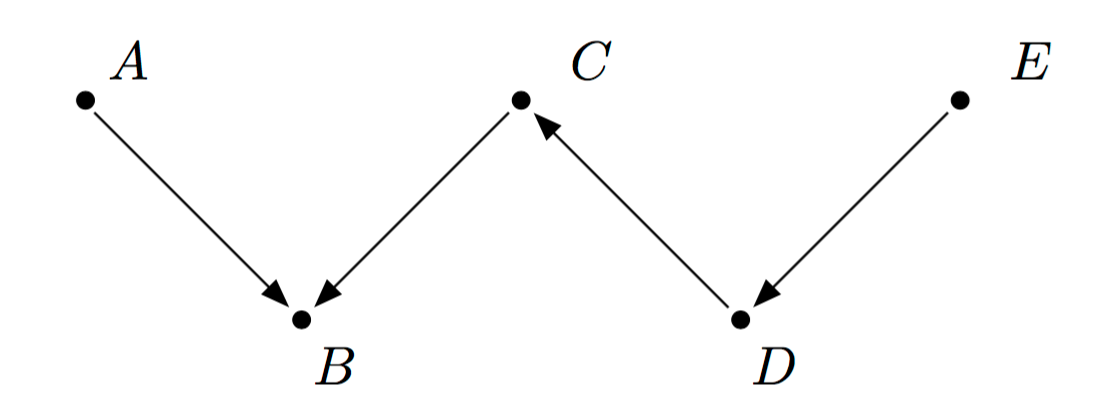
\includegraphics[height=3cm]{bayes1.png}
	\label{bayes1}
	\caption{Przykładowa sieć Bayesowska}
\end{figure}

Na rysunku został przedstawiony przykład nieskomplikowanej sieci Bayesowskiej. Na podstawie zaprezentowanego na rysunku grafu przedstawiającego sieć można wyciągnąć następujące wnioski:
\begin{itemize}
\item Para zmiennych A oraz B jest od siebie bezpośrednio zależna.
\item Para zmiennych B oraz C jest od siebie bezpośrednio zależna.
\item Zmienna reprezentowana przez wierzchołek B jest jednocześnie zależna od A oraz C.
\item Zmienne A oraz C pozostają brzegowo niezależne do momentu ustalenia wartości B (własność tą można również określić mówiąc, że zmienne A i C są d-połączone).
\item Zmienne E oraz C są zależne pośrednio.
\item Zmienna D d-separuje zmienne C i E.
\item Zmienne C i D d-separują parę zmiennych B, E.
\end{itemize}

\textbf{Orientacja łuków jest konieczna do określenia zależności nieprzechodnich.} Na przytoczonym przykładzie można zaobserwować, że pomimo faktu przemienności własności zależności orientacja krawędzi wnosi istotną informację o rozkładzie.\newline

Sieć Bayesowska pozwala na wyznaczenie rozkładu prawdopodobieństwa zmiennych. Jeżeli przez \(\Pi\)(Xi) oznaczymy zbiór rodziców danego wierzchołka w grafie, to rozkład prawdopodobieństwa zmiennych danej sieci opisuje się równaniem:
$$ P(X_{1}, X_{2}, ... , X_{n}) = \prod _{i=1}^{n}P(X_{i} | \Pi (X_{i})) $$

Co dla przedstawionego powyżej przykładu wynosi:
$$ P(A,B,C,D,E) = P(A)P(B|A,C)P(C|D)P(D|E)P(E) $$ 

Dzięki powyższemu równaniu równania możliwe jest określenie prawdopodobieństwa wystąpienia określonego wartościowania wszystkich zmiennych, znając jedynie lokalne prawdopodobieństwa warunkowe. Określając wartości tzw. \textit{przyczyn podstawowych}, czyli węzłów grafu nie posiadających rodziców (zmienne A, E w podanym przykładzie), można określić wartości oczekiwane innych atrybutów. Wszystkie pozostałe zmienne zależą bowiem pośrednio lub bezpośrednio od tego zbioru.

Istotą działania sieci Bayesowskich jest propagacja informacji o rozkładzie prawdopodobieństwa. 
W praktyce jednak \textbf{sieci Bayesowskie używane są do ekstrakcji informacji o rozkładach nieznanych, o których wiadomości możemy czerpać tylko z dostępnych wyników prób z eksperymentów statystycznych.} Sieci te nie są zatem używane do opisywania dokładnych rozkładów.

Próby z eksperymentów statystycznych (zestawy danych uczących) mogą mieć bardzo duże rozmiary, a ekstrakcja zawartych w nich w nich informacji może być zadaniem bardzo złożonym obliczeniowo. Proces uczenia sieci może być zatem postrzegany jako statystyczna kompresja informacji o rozkładzie do zwartej i jednocześnie bardziej przydatnej do wnioskowania bayesowskiego postaci.

Konstruowanie sieci Bayesowskiej składa się z następujących kroków:
\begin{itemize}
\item zdefiniowanie zmiennych,
\item zdefiniowanie połączeń pomiędzy zmiennymi,
\item określenie prawdopodobieństw warunkowych \textit{a priori}
\item wprowadzenie danych do sieci,
\item uaktualnienie sieci,
\item wyznaczenie prawdopodobieństw \textit{a posteriori}
\end{itemize}

Uczenie sieci jest uczeniem bez nadzoru i bez wstępnej wiedzy eksperckiej, a co za tym idzie zakłada się, że na wstępie (bez znajomości próby statystycznej) wszystkie dozwolone struktury sieci są jednakowo prawdopodobne, a przy ustalonej strukturze grafu wszystkie możliwe poprawne zbiory tablic prawdopodobieństw warunkowych są jednakowo prawdopodobne.

\subsubsection{Algorytm Chow-Liu}
Algorytm Chow-Liu stanowi klasyczny algorytm odtwarzający kształt zależności w próbie. Algorytm nie buduje sieci Bayesowskiej, a jedynie niezorientowane drzewo zależności. Jeżeli sieć Bayesa danego rozkładu ma postać drzewa, to algorytm Chow-Liu poprawnie odtworzy jego kształt. Algorytm Chow-Liu nie sprawdza, czy rozkład zmiennych zadanej próby D spełnia powyższy warunek. Jeśli struktura zależności między zmiennymi w próbie nie jest drzewem, to algorytm znajduje najlepszą strukturę drzewiastą, która opisuje postać zależności. Należy jednak pamiętać, że w skrajnie niekorzystnych wypadkach informacja zwrócona przez algorytm może być błędna.\newline

\textbf{Przebieg algorytmu:}\newline
\textbf{Krok 1:} Niech G oznacza graf pełny o zbiorze wierzchołków tożsamym ze zbiorem atrybutów próby D. Wówczas niech T będzie nieskierowaną strukturą drzewiastą uzyskaną w wyniku zastosowania dowolnego algorytmu znajdowania minimalnego drzewa rozpinającego (MST) w grafie G z funkcją wagową określającą stopień zależności między zmiennymi.\newline
\textbf{Krok 2:} W drzewie T należy obrać kierunki w sposób dowolny, uzyskując wynikową strukturę sieci Bayesa BS.\newline

W pierwszym kroku możliwe jest wykorzystanie odległości Kullback-Leiblera jako funkcji wagowej:
$$ DEP(X_{i}, X_{j}) = \sum_{x_{i}, x_{j}}^{ }  P(x_{i}, x_{j}) log \frac{P(x_{i}, x_{j})}{P(x_{i})P(x_{j})} $$

\begin{figure}[h!]
	\centering
	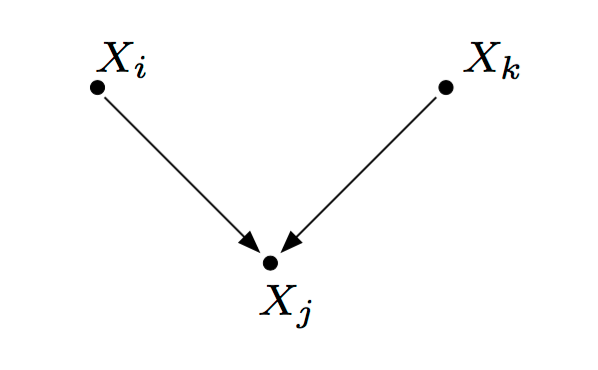
\includegraphics[height=3cm]{bayes2.png}
	\label{bayes2}
	\caption{Dwu rodziców: \(DEP(X_{i},X_{k}) = 0 \wedge DEP(X_{i},X_{k}|X_{j}) > 0\)}
\end{figure}

\begin{figure}[h!]
	\centering
	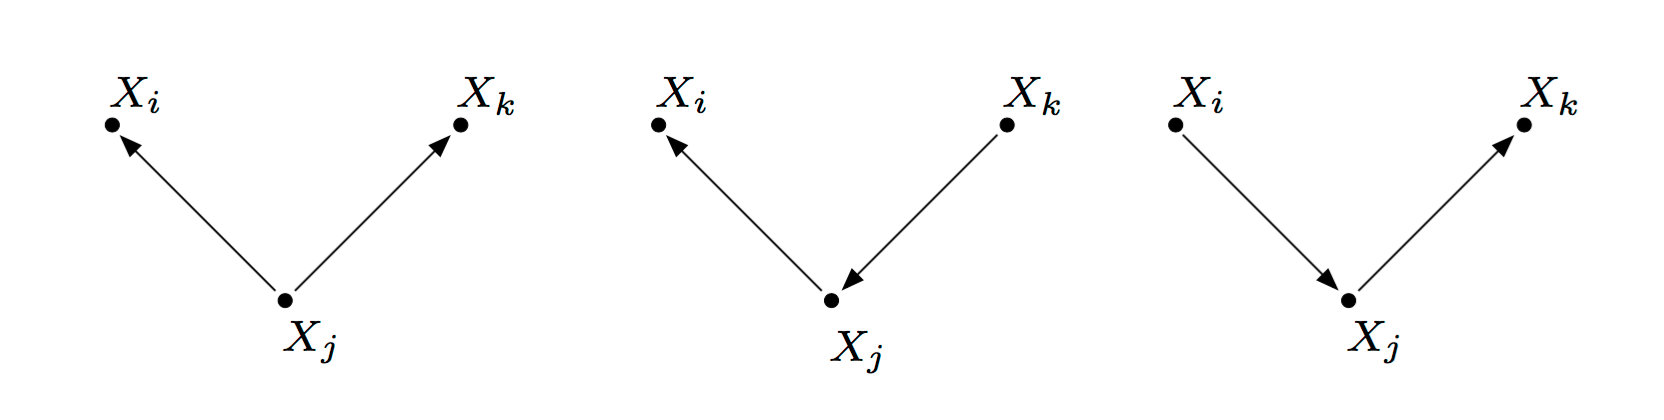
\includegraphics[height=3cm]{bayes3.png}
	\label{bayes3}
	\caption{\( X_{j}\) d-separuje \(X_{i},X_{k}:DEP(X_{i},X_{k})>0 \wedge DEP(X_{i},X_{k}|X_{j})=0\)}
\end{figure}

Gdzie podobnie jak w warunku małe litery \(x_{i}, x_{j}\) oznaczają wartościowania zmiennych \(X_{i}, X_{j} \)a sumowanie przebiega po wszystkich wartościowaniach w próbie D.





\newpage
\newpage

\subsection{Ukryte modele Markowa}

\subsubsection{Wstęp}

Ukryte modele Markowa (ang. \textit{Hidden Markov Model}, w skrócie \textit{HMM}) jest określeniem zaawansowanego modelu statystycznego znajdującego obecnie zastosowanie w wielu dziedzinach inżynierskich, szczególnie tam, gdzie analizowane są zjawiska o charakterze sekwencji losowych zdarzeń jak na przykład mowa czy gesty. Termin ten został wprowadzony i opisany matematycznie w drugiej połowie lat sześćdziesiątych ubiegłego wieku przez Bauma i Petriego, zaś swą nazwę zawdzięcza podstawie matematycznej, na której się opiera - łańcuchowi Markowa, który to określony został przez rosyjskiego matematyka Andrieja Markowa.

\begin{wrapfigure}{R}{0.5\textwidth}
  \centering
  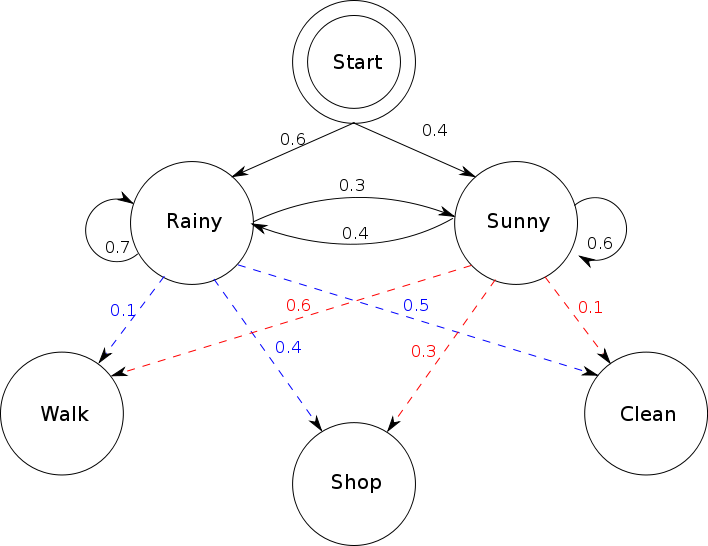
\includegraphics[width=0.5\textwidth]{markov.png}
  \caption{\label{fig:markov}Ogólny wygląd modelu Markowa.}
\end{wrapfigure}

W rozumieniu ogólnym ukryte modele Markowa określają system zdolny z pewnym prawdopodobieństwem przewidzieć jak zachowa się modelowany obiekt w przyszłości, bazując tylko i wyłącznie na jego aktualnym stanie, gdyż nie jest przechowywana historia wyników, jakie osiągał w przeszłości. Cały system dzieli się na niewidoczne dla obserwatora ukryte stany oraz część obserwowaną (wyjście), która jest losową funkcją stanu.

Dzięki swej rozbudowanej matematycznej charakterystyce, ukryte modele Markowa sukcesywnie stosowane są jako baza teoretyczna do rozwiązywania wielu problemów, a poprawnie zastosowane w praktyce dają bardzo dobre rezultaty. Głównymi zagadnieniami, przy których są one stosowane są modele akustyczne przy rozpoznawaniu mowy, rozpoznawanie pisma ręcznego, obiektów czy gestów. Znajdują zastosowanie również szeroko w bioinformatyce, biomedycynie, w psychologii do modelowania procesów uczenia się, w finansach przy modelowaniu ryzyka na rynku obligacji, przy prognozowaniu pogody, do generowania muzyki czy do wypełniania brakujących wyrazów w zdaniach. Jako ciekawe zastosowania wymienić również można modelowanie erupcji gejzeru \textit{Old Faithful} czy zbudowanie bota \textit{Mark V. Shaney} podszywającego się pod zwykłego użytkownika \textit{Usenetu} w latach osiemdziesiątych.

Jednym z głównych problemów występujących przy budowanie takiego modelu jest określenie odpowiedniego układu poprzez wyznaczenie topologii i dobranie wartości parametrów tak, aby otrzymać jak największą efektywność przy rozpoznawaniu. Klasyczne metody doboru parametrów modelu, jak algorytm \textit{Bauma-Welcha}, czy metody gradientowe, nie zapewniają znalezienia optymalnych wartości oraz wymagają poczynienia wstępnych założeń co do topologii modelu. Z tego to względu w ostatnich latach następuje znaczący wzrost zainteresowania tworzeniem nowych bądź udoskonalaniem obecnych metod budowy modelu.

\newpage

\subsubsection{Łańcuchy Markowa}

Łańcuchy Markowa najprościej określić można za pomocą jednej z dostępnych definicji. Wszystkie rozważania dotyczyć będą funkcji dyskretnej w czasie.

\begin{figure}[h!]
	\centering
	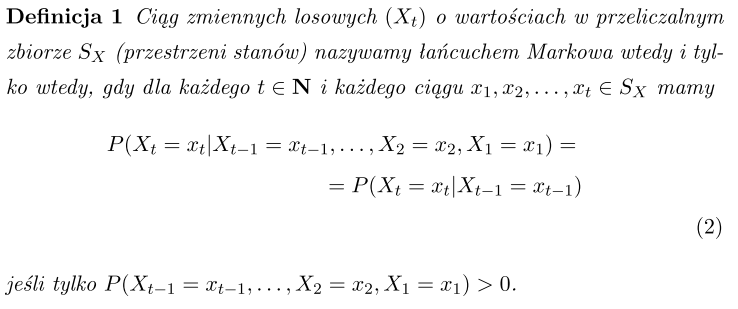
\includegraphics[width=0.80\linewidth]{definicja.PNG}
	\label{definicja}
\end{figure}

Warunek w powyższej definicji określa cały charakter łańcuchów Markowa, czyli, że ewolucja procesu zależy tylko i wyłącznie od bieżącego stanu. Zatem na charakter zmiennej $X_t$ w zadanej chwili $t$ ma wpływ wartość procesu w chwili $t - 1$. Taki łańcuch nazywamy łańcuchem Markowa rzędu pierwszego, czyli jego stan zależy tylko od stanu poprzedniego. Istnieją także rzędy \textit{x}, mówiące, że stan zależy od \textit{x}-stanów poprzednich.

W wypadku, gdy prawdopodobieństwa przejścia między stanami nie zależą od momentu, w którym rozpatrywany jest proces, wtedy łańcuch określić można mianem jednorodnego w czasie. Prawdopodobieństwo takie oznacza się jako $p_{ij}$. Macierz kwadratowa $P=[p_{ij}]$ jednorodnego łańcucha Markowa określa się jako macierz przejść.

\subsubsection{Definicja ukrytego modelu Markowa}

Dla rozważań w tym rozdziale, niech:

\begin{description}
  \item[T] = długość obserwowanej sekwencji
  \item[N] = liczba stanów w modelu
  \item[M] = liczba obserwacji
\end{description}

Mając na uwadze, że ukryty model Markowa jest szczególnym przypadkiem łańcuchu Markowa, możemy teraz opisać ten układ. Przejścia między stanami opisane niech będą przy pomocy kwadratowej macierzy prawdopodobieństw $A=[a_{ij}]$, gdzie element $a_{ij}$ jest to prawdopodobieństwo przejścia od stanu $i$ do stanu $j$ w następnej chwili czasowej.

$$ a_{ij}=Pr(x_{t}=j\,|\,x_{t-1}=i) \quad dla \quad 1 \leq i,j \leq N $$

Spełniona jest równość:

$$ \sum_{j=1}^{N} a_{ij} = 1 $$

\newpage

Kolejną składową systemu jest macierz $\Pi$ zawierająca prawdopodobieństwa wystąpienia \textbf{i}-tego stanu na początku sekwencji stanów.

$$ \Pi_{i} = Pr(x_{0}=1) $$

Znając obie macierze A oraz $\Pi$ można obliczyć prawdopodobieństwo wygenerowania przez system sekwencji stanów $X=(x_{0},x_{1}, \dots, x_{T})$.

$$ Pr(x\,|\,A,\Pi) = \Pi_{x_{0}}a_{x_{0}x_{1}}a_{x_{1}x_{2}} \dots x_{x_{T-1}x_{T}} $$

Tak opisana została warstwa ukryta. Model ten posiada jednakże jeszcze drugą warstwę, określaną mianami warstwy ukrytej, obserwowanej, bądź emisji. Każdemu ze stanów ukrytych przypada pewne prawdopodobieństwo $b$, mówiące, że w trakcie przebywania w nim, wygenerowana zostanie obserwacja $O_{t}$.

$$ B=\{b_{i}(O_{t})\}_{i=1}^{N} $$

Posiadając te wszystkie informacje można określić ukryty model Markowa jako $\lambda$:

$$ \lambda = (\Pi,A,B) $$

Teraz można obliczyć prawdopodobieństwo wygenerowania sekwencji obserwacji $O$ przez system $\lambda$:

$$ Pr(O\,|\,\Pi,A,B) = \sum_{x}P(O,x\,|\,\Pi,A,B) = \sum_{x}\Pi_{x_{0}}\prod_{t=1}^{T}a_{x_{t-1}x_{t}}b_{x_{t}}(O_{t}) $$

Ukryty model Markowa najprościej jest zobrazować przy pomocy poniższego schematu, zwanego grafem \textit{Trellisa}, gdyż ukazuje zmienność procesu wraz z czasem. Linią kropkowaną oddzielono to co widoczne jest przez obserwatora od warstwy ukrytej. Strzałki między węzłami mówią o bezpośredniej zależności stochastycznej, zaś brak strzałki oznacza niezależność losową.

\begin{figure}[h!]
	\centering
	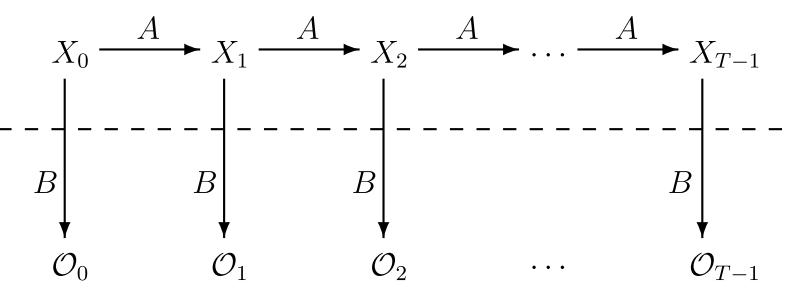
\includegraphics[width=0.70\linewidth]{markov-model.PNG}
	\label{markov-model}
	\caption{Ukryty model Markowa}
\end{figure}

Gdzie:

\begin{description}
  \item[X] = ($X_0, X_1, ..., X_{T-1}$) ukryte stany
  \item[O] = ($O_0, O_1, ..., O_{T-1}$) sekwencja obserwacji
  \item[A] = macierz prawdopodobieństw przejść między stanami
  \item[B] = macierz prawdopodobieństw wystąpienia obserwacji (emisji)
\end{description}

    \newpage

\section{Opis przeprowadzonych badań}

\subsection{Sieci Bayesowskie}
Badania przeprowadzone na zaimplementowanych sieciach bayesowskich miały za zadanie określenie różnic w działaniu modelu wynikających z zastosowania różnych algorytmów konstruowania sieci.\newline
Algorytmami wybranymi do przeprowadzenia badań były:
\begin{enumerate}
\item Algorytm naiwny
\item Algorytm Chow–Liu
\item Algorytm ,,Hill Climber''
\item Algorytm symulowanego wyżarzania
\item Algorytm ,,LAGD Hill Climber''
\end{enumerate}
Przeprowadzenie badań zostało rozpoczęte od utworzenia sieci bayesowskich korzystających z wymienionych powyżej algorytmów w do utworzenia struktury grafu.\newline
Następnie utworzone sieci bayesowskie poddano uczeniu za pomocą fragmentu zbioru danych dotyczącego występowania nawrotu choroby nowotworowej piersi pochodzącego z repozytorium \textit{UCI}\footnote{Link do zbioru: \url{https://archive.ics.uci.edu/ml/datasets/Breast+Cancer}}. Wspomniany zbiór składa się z zestawu dziewięciu cech opisywanych wartościami dyskretnymi oraz dwóch klas.\newline
Przed rozpoczęciem procesu uczenia atrybuty zbioru uczącego zostały przekonwertowane na format ,,One Hot Encoding'' (OHE). \newline
Po zakończeniu procesu uczenia na wejście modeli został podany fragment zbioru danych rozłączny ze zbiorem wykorzystanym do uczenia. Na podstawie danych otrzymanych w wyniku predykcji dokonywanych przez modele obliczony został ich błąd klasyfikacji. Co więcej, dla każdego algorytmu generowania sieci sporządzono macierz błędów (tablicę pomyłek).  \newline
Na podstawie opracowanej macierzy błędów wyznaczone zostały miary jakości modeli:
\begin{itemize}
\item prawdziwie pozytywna (ang. true positive TP)
\item prawdziwie negatywna (ang. true negative TN)
\item fałszywie pozytywna (ang. false positive FP), błąd I typu
\item fałszywie negatywna (ang. false negative FN), błąd II typu
\item czułość (ang. sensitivity) - odsetek prawdziwie pozytywnych (ang. true positive rate TPR)
\item specyficzność (ang. specificity SPC) - odsetek prawdziwie negatywnych (ang. True Negative Rate TNR)
\item precyzja (ang. precision)
\item dokładność (ang. accuracy ACC)
\end{itemize}
\vspace{5mm}
\textbf{\textit{Czułość}}  interpretuje się jako zdolność modelu do prawidłowego rozpoznania nawrotu choroby tam, gdzie on występuje i została obliczone zgodnie ze wzorem:
$$ TPR = TP/(TP+FN) $$
Gdzie:\\
TPR - czułość\\
TP -  prawdziwie pozytywna\\
FN - fałszywie negatywna\\
Czułość 100\% oznaczałaby, że wszystkie osoby z nawrotem choroby zostaną wyznaczone przez model.\\
\vspace{5mm}
\textbf{\textit{Specyficzność}} wyznaczono na podstawie równania:
$$ TNR = TN/(FP+TN) $$
Gdzie:\\
TNR - specyficzność \\
TN - prawdziwie negatywna\\
FP - fałszywie pozytywna\\
Specyficzność 100\% oznaczałaby, że wszyscy ludzie zdrowi w wykonanym teście  zostaną oznaczeni przez model jako zdrowi.\\

\textbf{\textit{Precyzja}} jest określona wzorem:
$$ PRE = TP/(TP+FP) $$
Gdzie:\\
PRE - precyzja\\
TP -  prawdziwie pozytywna\\
FP -  fałszywie pozytywna\\

\textbf{\textit{Dokładność}} obliczono korzystając z równania:
$$ ACC = (TP+TN)/(P+N) $$
Gdzie:\\
ACC -  dokładność\\
TP -  prawdziwie pozytywna\\
TN -  prawdziwie negatywna\\
P -  wartości wyznaczone poprawnie\\
N -  wartości wyznaczone błędnie\\

Dodatkowo wygenerowane zostały grafy przedstawiające strukturę sieci bayesowskiej analizowanych modeli, dzięki czemu możliwe było bardziej szczegółowe przeanalizowanie wyników.

Na koniec wykonane zostały także symulacje działania klasyfikatorów:
\begin{itemize}
\item Sieci neuronowej z wsteczną propagacją błędów
\item Sieci neuronowej typu ELM
\item Support Vector Machine
\end{itemize}
na tym samym zbiorze danych. Dzięki temu możliwe było odniesienie otrzymanych przez sieci bayesowskie wyników do rezultatów osiąganych przez inne rodzaje klasyfikatorów.
\newpage


\subsubsection{Sieć bayesowska otrzymana za pomocą algortymu ,,Hill Climber''}

\begin{table}[H]
\centering
\caption{Macierz błędu sieci bayesowskiej otrzymanej za pomocą algortymu ,,Hill Climber''}
\label{my-label}
\begin{tabular}{
>{\columncolor[HTML]{FFFFFF}}c 
>{\columncolor[HTML]{FFFFFF}}c |c|c|}
\cline{3-4}
\multicolumn{2}{c}{\cellcolor[HTML]{FFFFFF}}                                                                          & \multicolumn{2}{c|}{\cellcolor[HTML]{9B9B9B}Klasa przewidywana}                                                     \\ \cline{3-4} 
\multicolumn{2}{c}{\multirow{-2}{*}{\cellcolor[HTML]{FFFFFF}}}                                                        & \cellcolor[HTML]{C0C0C0}{\color[HTML]{333333} pozytywna} & \cellcolor[HTML]{C0C0C0}{\color[HTML]{333333} negatywna} \\ \hline
\multicolumn{1}{|c|}{\cellcolor[HTML]{9B9B9B}}                                    & \cellcolor[HTML]{C0C0C0}pozytywna & 4                                                        & 17                                                        \\ \cline{2-4} 
\multicolumn{1}{|c|}{\multirow{-2}{*}{\cellcolor[HTML]{9B9B9B}Klasa rzeczywista}} & \cellcolor[HTML]{C0C0C0}negatywna & 9                                                        & 28                                                        \\ \hline
\end{tabular}
\end{table}
\textbf{Miary jakości otrzymanych wyników:\\}
Poprawnie zaklasyfikowane:	32\\
Błędnie zaklasyfikowane:	26\\
Czułość:	30,77\%\\
Specyficzność:	62,22\%\\
Precyzja:	19,05\%\\
Dokładność:	55,17\%\\
Błąd:	44,83\%\\

\begin{figure}[H]
	\centering
	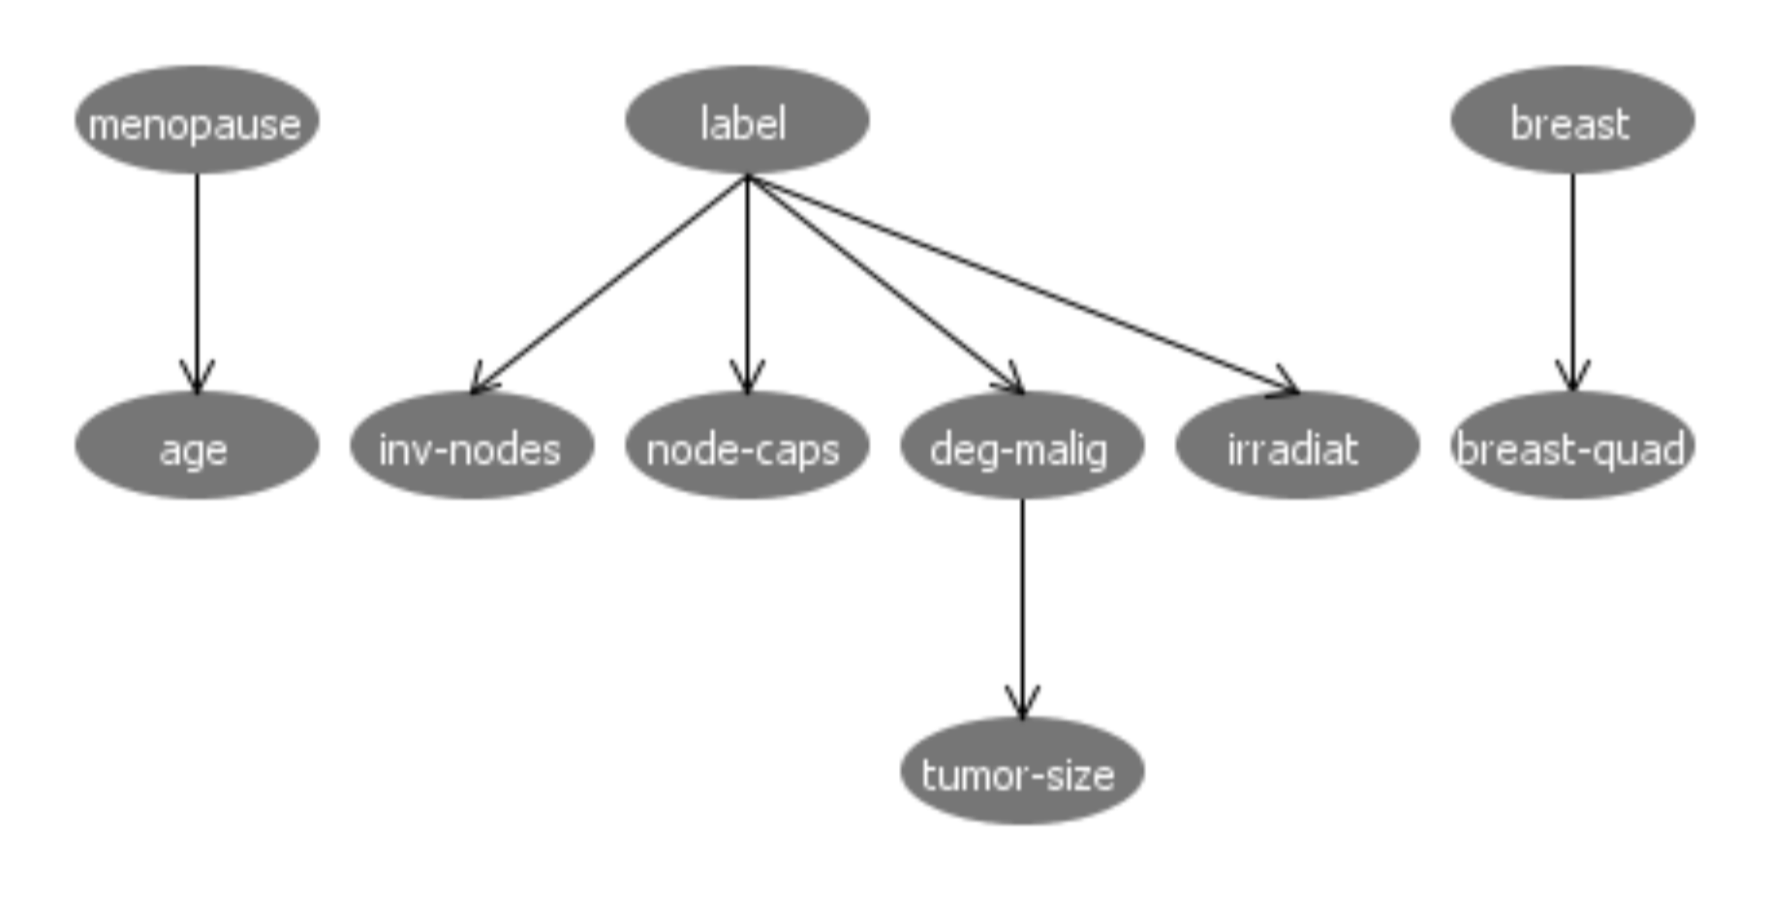
\includegraphics[width=0.70\linewidth]{hill-climber.png}
	\label{hc}
	\caption{Graf sieci bayesowskiej otrzymanej za pomocą algortymu ,,Hill Climber''}
\end{figure}

Algorytm Hill Climber charakteryzuje się umiejętnością znajdowania ekstremów lokalnych. Niestety podczas procesu optymalizacji ma tendencję do znajdowania przeciętnych rozwiązań , które wydają się obiecujące jedynie lokalnie. Prawdopodobnie właśnie dlatego otrzymane przez algorytm Hill Climber rozwiązanie charakteryzuje się niską dokładnością (55\% przy problemie dwuklasowym).\\abstractname{}  Warto zwrócić także uwagę na niską wartość precyzji oraz czułości. Istotną obserwacją jest fakt, że model znacznie częściej wybierał klasę negatywną, co prowadziło do zawyżenia wartości specyficzności i obniżenia czułości. \\
Wybór klasy negatywnej może wynikać ze zbytniego dopasowania się do zbioru uczącego, w wyniku czego prawdopodobieństwo przynależności do klasy pozytywnej wyliczane dla obiektów ze zbioru testowego było stosunkowo niskie.\\
Warto zauważyć, że algorytm bardzo dobrze poradził sobie ze znalezieniem prawidłowości występujących pomiędzy wiekiem pacjentki, a wiekiem wystąpienia u niej menopauzy oraz zależności pomiędzy piersią dotkniętą nowotworem, a kwartylem piersi (w zbiorze wystąpiła duplikacja informacji). Algorytmowi nie udało się zbudować więcej niż dwóch poziomów zależności przyczynowo skutkowych, co może być jedyną z przyczyn jego słabych wyników.

\subsubsection{Sieć bayesowska otrzymana za pomocą algorytmu symulowanego wyżarzania}

\begin{table}[H]
\centering
\caption{Macierz błędu sieci bayesowskiej otrzymanej za pomocą algorytmu symulowanego wyżarzania}
\label{my-label}
\begin{tabular}{
>{\columncolor[HTML]{FFFFFF}}c 
>{\columncolor[HTML]{FFFFFF}}c |c|c|}
\cline{3-4}
\multicolumn{2}{c}{\cellcolor[HTML]{FFFFFF}}                                                                          & \multicolumn{2}{c|}{\cellcolor[HTML]{9B9B9B}Klasa przewidywana}                                                     \\ \cline{3-4} 
\multicolumn{2}{c}{\multirow{-2}{*}{\cellcolor[HTML]{FFFFFF}}}                                                        & \cellcolor[HTML]{C0C0C0}{\color[HTML]{333333} pozytywna} & \cellcolor[HTML]{C0C0C0}{\color[HTML]{333333} negatywna} \\ \hline
\multicolumn{1}{|c|}{\cellcolor[HTML]{9B9B9B}}                                    & \cellcolor[HTML]{C0C0C0}pozytywna & 3                                                        & 18                                                        \\ \cline{2-4} 
\multicolumn{1}{|c|}{\multirow{-2}{*}{\cellcolor[HTML]{9B9B9B}Klasa rzeczywista}} & \cellcolor[HTML]{C0C0C0}negatywna & 7                                                        & 30                                                        \\ \hline
\end{tabular}
\end{table}

\textbf{Miary jakości otrzymanych wyników:\\}
Poprawnie zaklasyfikowane:	33\\
Błędnie zaklasyfikowane:	25\\
Czułość:	30,00\%\\
Specyficzność:	62,50\%\\
Precyzja:	14,29\%\\
Dokładność:	56,90\%\\
Błąd:	43,10\%\\

\begin{figure}[H]
	\centering
	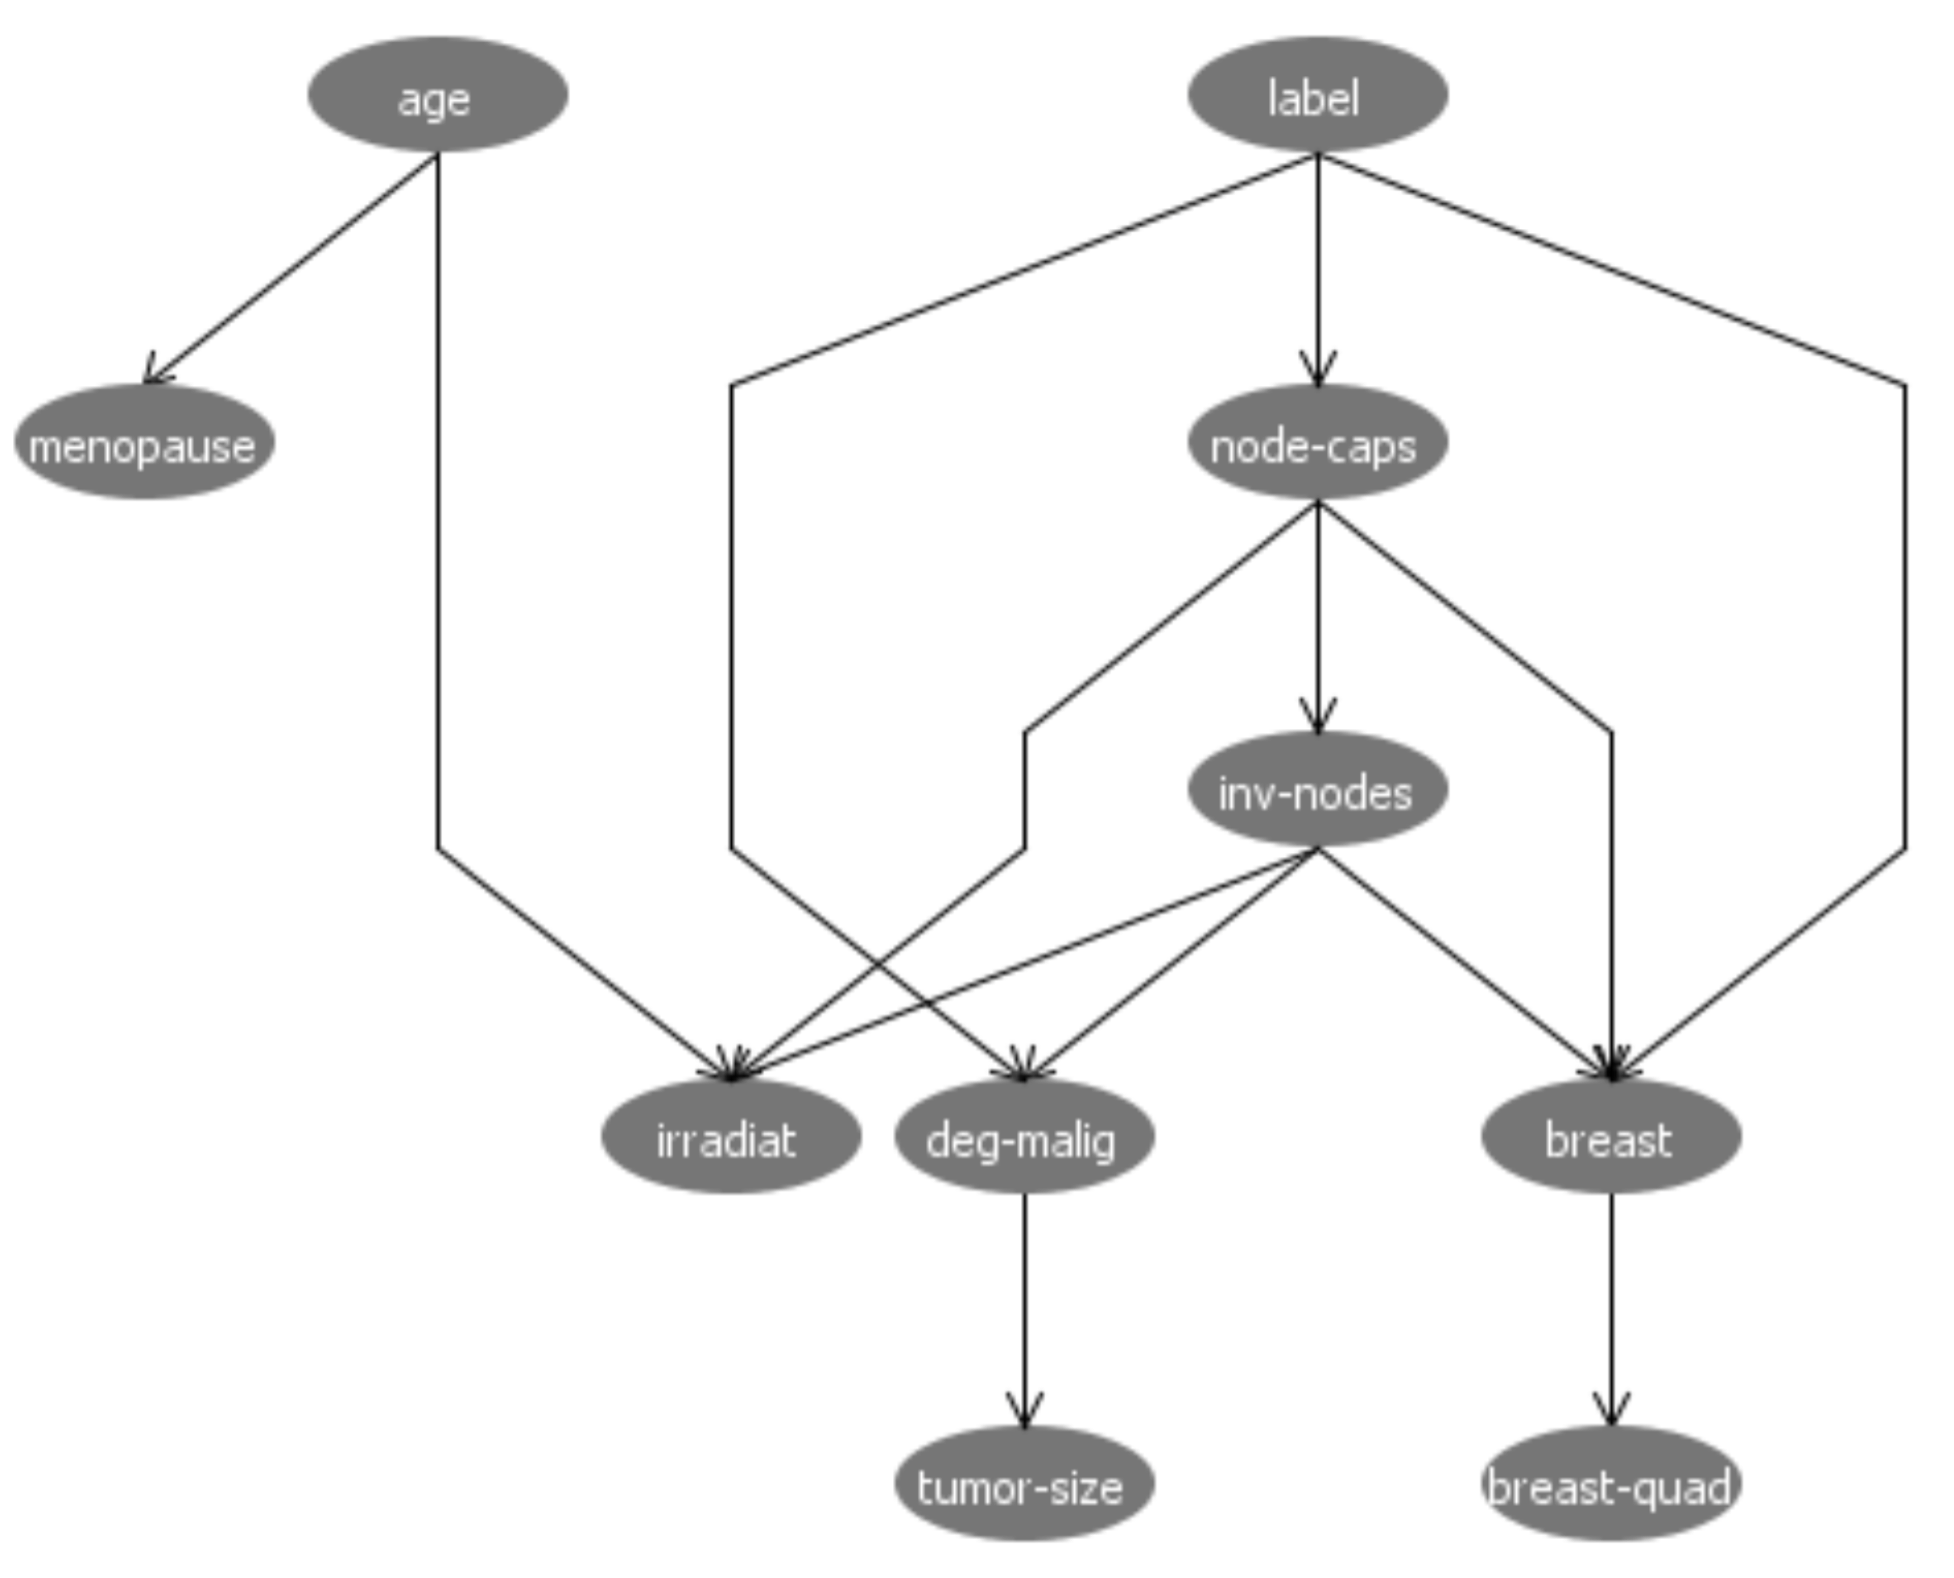
\includegraphics[width=0.70\linewidth]{simulated-annealing.png}
	\label{sa}
	\caption{Graf sieci bayesowskiej otrzymanej za pomocą algorytmu symulowanego wyżarzania}
\end{figure}

Algorytm symulowanego wyżarzania eliminuje podstawową wadę algorytmu Hill Climber - tendencję do utykania w ekstremum lokalnym. Algorytm poprzez wykonywanie skoków w losowe miejsca (prawdopodobieństwo określone rozkładem) w kolejnych iteracjach algorytmu. Zastosowanie bardziej skomplikowanej heurystyki zaowocowało uzyskaniem wyższej o około 1.73\% dokładności modelu.\\abstractname{}  Lekkiemu obniżeniu uległa precyzja, a pozostałe metryki pozostały na zbliżonym poziomie.  Graf skonstruowany przez algorytm symulowanego wyżarzania charakteryzuje się znacznie większą liczbą znalezionych zależności przyczynowo-skutkowych niż w przypadku poprzedniego algorytmu. \\
Dodatkowo graf zawiera znacznie mniej liści, co może sugerować, że niektóre zależności  mogą być nieprawidłowe - zgodnie z grafem dwa stany są pośrednio lub bezpośrednio zależne od pięciu innych. Być może ta właściwość grafu doprowadziła do niskiej skuteczności klasyfikatora. 

\subsubsection{Sieć bayesowska otrzymana za pomocą algortymu ,,LAGD Hill Climber''}

\begin{table}[H]
\centering
\caption{Macierz błędu sieci bayesowskiej otrzymanej za pomocą algorytmu ,,LAGD Hill Climber''}
\label{my-label}
\begin{tabular}{
>{\columncolor[HTML]{FFFFFF}}c 
>{\columncolor[HTML]{FFFFFF}}c |c|c|}
\cline{3-4}
\multicolumn{2}{c}{\cellcolor[HTML]{FFFFFF}}                                                                          & \multicolumn{2}{c|}{\cellcolor[HTML]{9B9B9B}Klasa przewidywana}                                                     \\ \cline{3-4} 
\multicolumn{2}{c}{\multirow{-2}{*}{\cellcolor[HTML]{FFFFFF}}}                                                        & \cellcolor[HTML]{C0C0C0}{\color[HTML]{333333} pozytywna} & \cellcolor[HTML]{C0C0C0}{\color[HTML]{333333} negatywna} \\ \hline
\multicolumn{1}{|c|}{\cellcolor[HTML]{9B9B9B}}                                    & \cellcolor[HTML]{C0C0C0}pozytywna & 3                                                        & 18                                                        \\ \cline{2-4} 
\multicolumn{1}{|c|}{\multirow{-2}{*}{\cellcolor[HTML]{9B9B9B}Klasa rzeczywista}} & \cellcolor[HTML]{C0C0C0}negatywna & 3                                                        & 34                                                        \\ \hline
\end{tabular}
\end{table}

\textbf{Miary jakości otrzymanych wyników:\\}
Poprawnie zaklasyfikowane:	37\\
Błędnie zaklasyfikowane:	21\\
Czułość:	50,00\%\\
Specyficzność:	65,38\%\\
Precyzja:	14,29\%\\
Dokładność:	63,79\%\\
Błąd:	36,21\%\\

\begin{figure}[H]
	\centering
	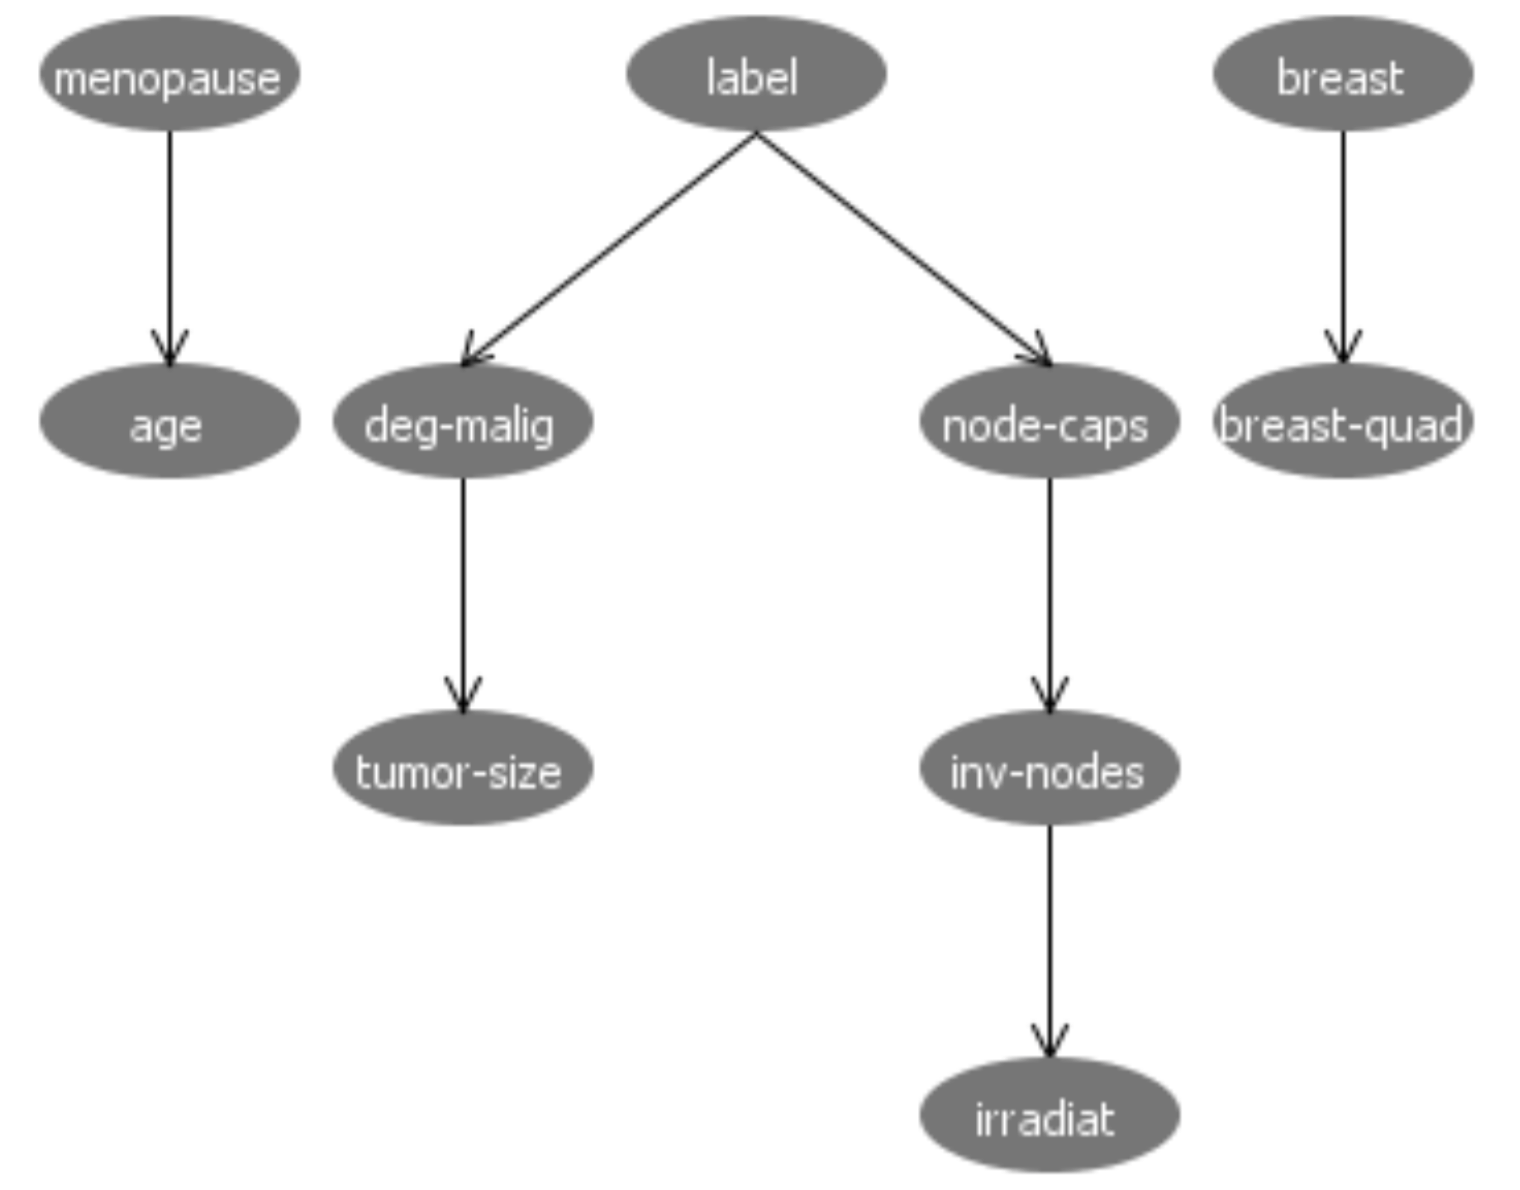
\includegraphics[width=0.55\linewidth]{lagd-hill-climber.png}
	\label{lagdhc}
	\caption{Graf sieci bayesowskiej otrzymanej za pomocą algorytmu ,,LAGD Hill Climber''}
\end{figure}

Algorytm LAGD Hill Climber stanowi rozszerzenie algorytmu Hill Climber polegające na analizie dodatkowo kilku kroków algorytmu wprzód w celu odnalezienia najlepszej struktury grafu. Dzięki zastosowaniu wspomnianego usprawnienia udało się otrzymać dokładność klasyfikacji wyższą o około 8,5\%, co stanowi świetny rezultat. \\
Powstały graf ma podobną strukturę do grafu powstałego w efekcie działania Hill Climber. Zmianie uległo największe drzewo grafu, a pozostałe dwa mniejsze pozostały bez zmian.  \\
Nowa struktura największego drzewa posiada dwukrotnie mniej liści, co sugeruje, że  udało się odszukać głębsze zależności między stanami. Otrzymany graf stanowi formę pośrednią pomiędzy poprzednimi dwoma strukturami. \\
Otrzymany model w porównaniu do poprzedników charakteryzuje się wysoką czułością, ponieważ  lepiej radzi sobie z prawidłowym rozpoznaniem nawrotu choroby.


\subsubsection{Sieć bayesowska otrzymana za pomocą algorytmu naiwnego}
\begin{table}[H]
\centering
\caption{Macierz błędu sieci bayesowskiej otrzymanej za pomocą algorytmu naiwnego}
\label{my-label}
\begin{tabular}{
>{\columncolor[HTML]{FFFFFF}}c 
>{\columncolor[HTML]{FFFFFF}}c |c|c|}
\cline{3-4}
\multicolumn{2}{c}{\cellcolor[HTML]{FFFFFF}}                                                                          & \multicolumn{2}{c|}{\cellcolor[HTML]{9B9B9B}Klasa przewidywana}                                                     \\ \cline{3-4} 
\multicolumn{2}{c}{\multirow{-2}{*}{\cellcolor[HTML]{FFFFFF}}}                                                        & \cellcolor[HTML]{C0C0C0}{\color[HTML]{333333} pozytywna} & \cellcolor[HTML]{C0C0C0}{\color[HTML]{333333} negatywna} \\ \hline
\multicolumn{1}{|c|}{\cellcolor[HTML]{9B9B9B}}                                    & \cellcolor[HTML]{C0C0C0}pozytywna & 0                                                        & 18                                                        \\ \cline{2-4} 
\multicolumn{1}{|c|}{\multirow{-2}{*}{\cellcolor[HTML]{9B9B9B}Klasa rzeczywista}} & \cellcolor[HTML]{C0C0C0}negatywna & 0                                                        & 40                                                        \\ \hline
\end{tabular}
\end{table}
\textbf{Miary jakości otrzymanych wyników:\\}
Poprawnie zaklasyfikowane:	40\\
Błędnie zaklasyfikowane:	18\\
Czułość:	niemożliwa do wyznaczenia\\
Specyficzność:	68,97\%\\
Precyzja:	0,00\%\\
Dokładność:	68,97\%\\
Błąd:	31,03\%\\

\begin{figure}[H]
	\centering
	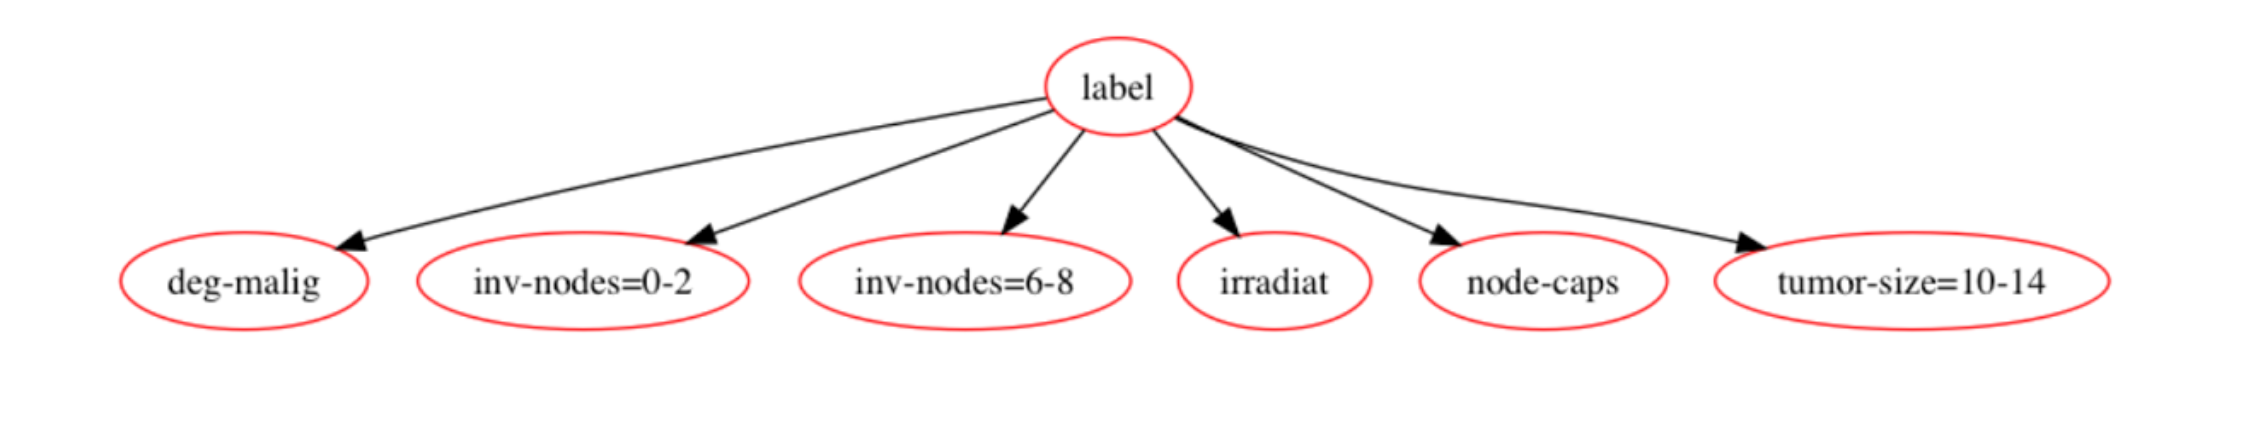
\includegraphics[width=0.80\linewidth]{naive3.png}
	\label{hc}
	\caption{Graf sieci bayesowskiej otrzymanej za pomocą algorytmu naiwnego}
\end{figure}

Sieć bayesowska skonstruowana za pomocą algorytmu naiwnego składa się  drzewa (korzeń i liście). Ze względu na to, że algorytmowi naiwnemu nie udało się odszukać zbyt wielu zależności przyczynowo skutkowych w zbiorze model posiada znikomą wartość jako klasyfikator. \\
W ramach testów przeprowadzonym na zbiorze testowym wszystkie otrzymane odpowiedzi były takie same - 'no-reccurence-events'. W związku z tym precyzja modelu wyniosła 0\%. Wysoka w porównaniu z poprzedniki algorytmami skuteczności jest jedynie dziełem przypadku i wynika z proporcji klas w zbiorze testowym. Wnioskiem z przeprowadzonego eksperymentu jest fakt, że algorytm naiwny może okazać się zbyt prosty aby odpowiednio odwzorować zależności występujące w zbiorze w postaci grafu.

\subsubsection{Sieć bayesowska otrzymana za pomocą algortymu Chow-Liu}
\begin{table}[H]
\centering
\caption{Macierz błędu sieci bayesowskiej otrzymanej za pomocą algortymu Chow-Liu}
\label{my-label}
\begin{tabular}{
>{\columncolor[HTML]{FFFFFF}}c 
>{\columncolor[HTML]{FFFFFF}}c |c|c|}
\cline{3-4}
\multicolumn{2}{c}{\cellcolor[HTML]{FFFFFF}}                                                                          & \multicolumn{2}{c|}{\cellcolor[HTML]{9B9B9B}Klasa przewidywana}                                                     \\ \cline{3-4} 
\multicolumn{2}{c}{\multirow{-2}{*}{\cellcolor[HTML]{FFFFFF}}}                                                        & \cellcolor[HTML]{C0C0C0}{\color[HTML]{333333} pozytywna} & \cellcolor[HTML]{C0C0C0}{\color[HTML]{333333} negatywna} \\ \hline
\multicolumn{1}{|c|}{\cellcolor[HTML]{9B9B9B}}                                    & \cellcolor[HTML]{C0C0C0}pozytywna & 0                                                        & 15                                                        \\ \cline{2-4} 
\multicolumn{1}{|c|}{\multirow{-2}{*}{\cellcolor[HTML]{9B9B9B}Klasa rzeczywista}} & \cellcolor[HTML]{C0C0C0}negatywna & 1                                                        & 42                                                        \\ \hline
\end{tabular}
\end{table}
\textbf{Miary jakości otrzymanych wyników:\\}
Poprawnie zaklasyfikowane:	42\\
Błędnie zaklasyfikowane:	16\\
Czułość:	0,00\%\\
Specyficzność:	73,68\%\\
Precyzja:	0,00\%\\
Dokładność:	72,41\%\\
Błąd:	27,59\%\\

\begin{figure}[H]
	\centering
	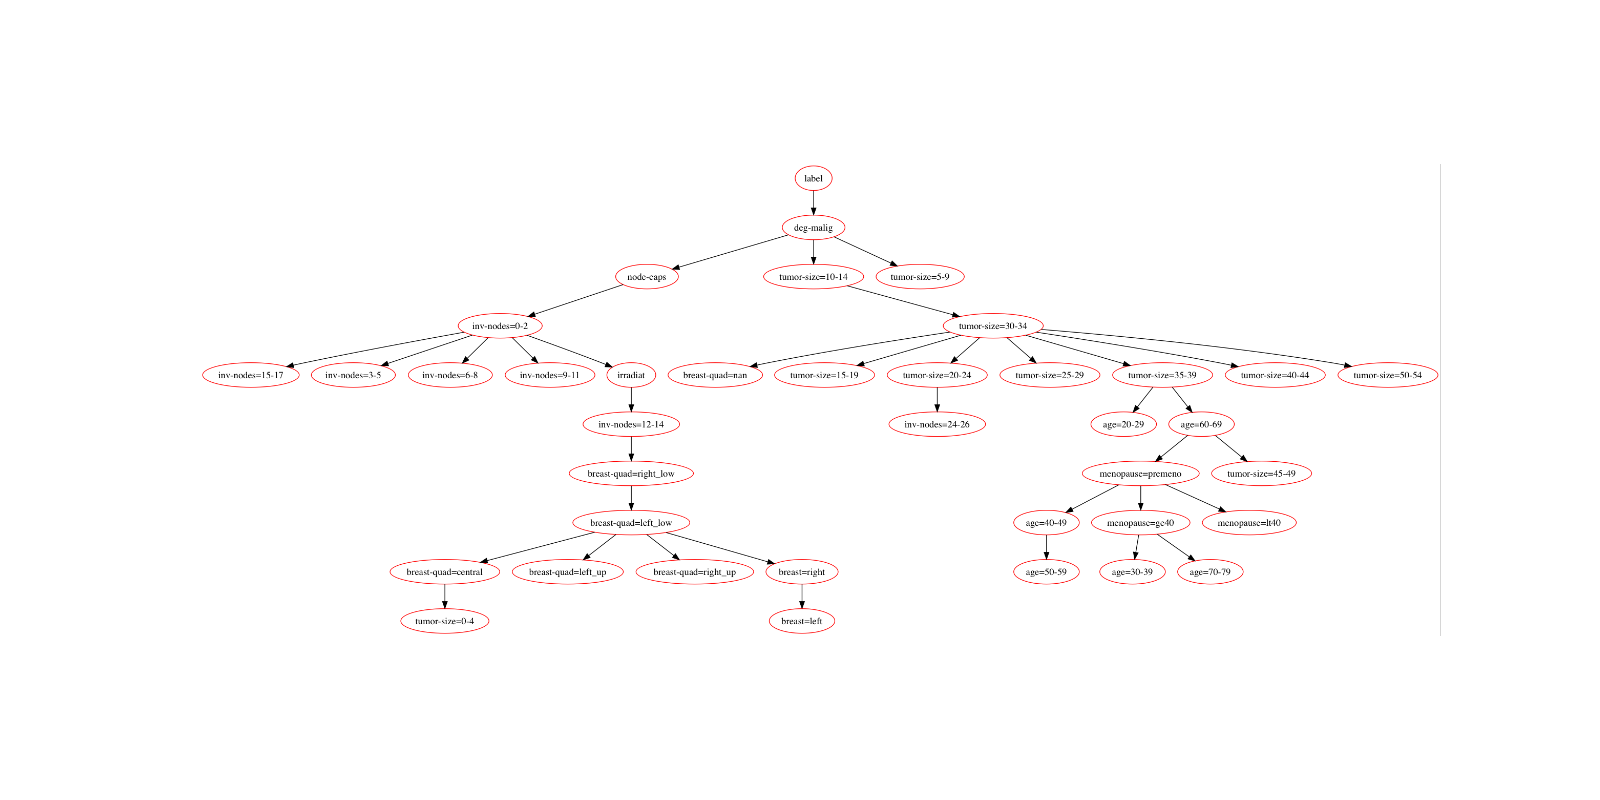
\includegraphics[width=0.97\linewidth]{chow-liu.png}
	\label{hc}
	\caption{Graf sieci bayesowskiej otrzymanej za pomocą algortymu Chow-Liu}
\end{figure}

Cechą algorytmu Chow-Liu jest fakt, że produkuje on niezorientowane drzewo zależności. Jeżeli sieć Bayesa danego rozkładu ma postać drzewa, to algorytm Chow-Liu poprawnie odtworzy jego kształt. Algorytm Chow-Liu nie sprawdza, czy rozkład zmiennych zadanej próby spełnia powyższy warunek. \\
Jeśli struktura zależności między zmiennymi w próbie nie jest drzewem, to algorytm znajduje najlepszą strukturę drzewiastą, która opisuje postać zależności. Należy pamiętać, że w  niekorzystnych wypadkach informacja zwrócona przez algorytm może być błędna. \\
Tak właśnie stało się w przypadku  analizowanego przez nas zbioru danych. Już po samej strukturze grafu widać, że znalezione przez algorytm zależności przyczynowo-skutkowe są niepoprawne. Przykładem niepoprawnej zależności może być  występowanie 6-8 ognisk nowotworu w przypadku występowania 0-2 ognisk nowotworu (wystąpienie tych sytuacji wzajemnie się wyklucza). \\
W efekcie otrzymany model nie nadaje się do wykorzystania w celach diagnostycznych, a wartości parametrów czułości i precyzji wynoszą 0\% pomimo wysokiej dokładności (72\%). Podobnie jak w przypadku algorytmu naiwnego, dokładność odwzorowała jedynie przybliżenie rozkładu klas w zbiorze uczącym.


\begin{table}[H]
\centering
\caption{Zestawienie dokładności klasyfikacji otrzymanej przez wszystkie modele uczestniczące w przeprowadzonym eksperymencie}
\label{last}
\begin{tabular}{|l|l|}
\hline
\rowcolor[HTML]{C0C0C0} 
{\color[HTML]{333333} Model}            & {\color[HTML]{333333} Dokładność klasyfikacji} \\ \hline
Sieć bayesowska (algorytm naiwny)       & 68.97\%                                        \\ \hline
Sieć bayesowska (Chow–Liu)              & 72.41\%                                        \\ \hline
Sieć bayesowska (,,Hill Climber”)       & 55,17\%                                        \\ \hline
Sieć bayesowska (symulowane wyżarzanie) & 56,90\%                                        \\ \hline
Sieć bayesowska (,„LAGD Hill Climber”)  & 63,79\%                                        \\ \hline
Sieć neuronowa z wsteczną propagacją    & 71,08\%                                        \\ \hline
Sieć neuronowa typu ELM                 & 69,97\%                                        \\ \hline
Support Vector Machine                  & 73,11\%                                        \\ \hline
\end{tabular}
\end{table}

Eksperymenty przeprowadzone na zestawie ośmiu modeli pokazują, że efekty uzyskane przez sieci bayesowskie są wyraźnie gorsze od bardziej skomplikowanych modeli. Wyniki uzyskane przez algorytm naiwny oraz Chow-Liu  zostały zignorowane ze względu na bardzo niskie miary jakości tych modeli. Spośród sieci bayesowskich najlepiej poradził sobie algorytm LAGD Hill Climber. Dzięki przewidywaniu na kilka kroków wprzód, która stryktura grafu może okazać się skuteczniejsza udało mu się poprawić wyniki klasycznego algorytmu Hill Climber o ponad 8\% c stanowi znaczącą różnicę. Algorytm symulowanego wyżarzania osiągnął poziom podobny do klasycznego algorytmu Hill Climber pokonując go o około 1,7\%. Sieć typu ELM ze względu na swoją uproszczoną strukturę uplasowała się poniżej sieci neuronowej ze wsteczną propagacją (jednak udało się jej uzyskać znacznie lepsze czasu uczenia).  Najlepszym klasyfikatorem okazał się SVM, któremu udało się osiągnąć rezultat lepszy o 10\% niż LAGD Hill Climber oraz około 18\% lepszy od pozostałych sieci bayesowskich.  

\newpage

\subsection{Ukryte modele Markowa}

Badania dla ukrytego modelu Markowa przeprowadzono dla zobrazowania podstawowych zależności zachodzących między zbiorem podstawowym nie posiadającym żadnej wiedzy o problemie, czy w tym wypadku chorobie, oraz zbioru sekwencyjnego, taką wiedzę posiadającą. Ideą zbioru sekwencyjnego było aby składał się on z danych wskazujących w jaki sposób zmieniała się choroba wraz z czasem.

W projekcie wykorzystano zbiór charakteryzujący problem raka piersi z darmowego internetowego zasobu \textit{UCI}, który to nie posiadał historii choroby\footnote{Link do zbioru: \url{https://archive.ics.uci.edu/ml/datasets/Breast+Cancer}}. Należało zatem historię przemian wygenerować własnoręcznie. Posłużono się w tym celu macierzą przejść łańcucha Markowa, który przedstawiał prawdopodobieństwa przejścia od klasy \textit{X} do klasy \textit{Y}, bądź zostania dalej w klasie \textit{X}. Cały schemat generowania sekwencji przedstawić można w kilku krokach:
\\
\begin{enumerate}
  \item Stwórz macierz przejść łańcucha Markowa
  \item Posortuj próbki po klasie
  \item Dla każdej próbki:
    \begin{enumerate}
    \item Wybierz następną klasę z prawdopodobieństwem z macierzy
    \item Dla wybranej klasy wybierz próbkę z prawdopodobieństwem losowym
    \item Dopisz wybraną klasę i próbkę jako sekwencja
    \end{enumerate}
\end{enumerate}

\par
\bigskip

Posiadając oba zbioru - bazowy oraz sekwencyjny, przeprowadzono badania najważniejszych parametrów modelu - czasu uczenia, czasu testowania oraz efektywności. Manipulowano przy tym dostępnym parametrem - algorytmem dekodowania, gdzie starano się zbadać jaki wpływ na wyniki ma zmiana algorytmu. Zastosowano dwa algorytmy - algorytm Viterbiego bazujący na technice programowania dynamicznego, oraz algorytm heurystyczny "best-first" znany także jako algorytm dekodowania posteriori.

Jako stałe parametry przyjęto długość sekwencji na 2, gdyż wstępne badania wykazały, iż zwiększenie sekwencji nie wpływa w zauważalny sposób na wyniki. Niezmienny był także współczynnik zbioru testowego, wynoszący 0.2, co wskazywało, iż 20\% zbioru wejściowego wykorzystywane jest jako zbiór testowy. Następnym niezmiennym parametrem był parametr wejściowy do algorytmu - alfa, który to w literaturze angielskiej określany jest jako \textit{Lidstone (additive) smoothing parameter}, a jego zmiana również nie wpływała w zauważalny sposób na wyniki badań.

W celu oszczędzenie miejsca na poniższych wykresach skrócono nazewnictwo, które oznacza:

\begin{itemize}
  \item \textit{nonseq Viterbi} - Badanie przy użyciu zbioru bez sekwencji oraz algorytmu Viterbiego
  \item \textit{seq Viterbi} - Badanie przy użyciu zbioru z sekwencjami oraz algorytmu Viterbiego
  \item \textit{nonseq bestfirst} - Badanie przy użyciu zbioru bez sekwencji oraz algorytmu "best-first"
  \item \textit{seq bestfirst} - Badanie przy użyciu zbioru z sekwencjami oraz algorytmu "best-first"
\end{itemize}

Wszystkie badania powtórzono 100 razy i na podstawie wyników wyciągnięto podstawowe wartości statystyczne jak:

\begin{itemize}
  \item \textit{max} - wartość minimalna
  \item \textit{min} - wartość maksymalna
  \item \textit{mean} - wartość średnia
  \item \textit{std} - odchylenie standardowe
\end{itemize}

\newpage

Pierwszymi badaniami było sprawdzenie czasu uczenia modelu. Jak widać, czas uczenia nieznacząco rośnie o około 15\% jeśli chodzi o zbiór sekwencyjny względem zbioru bazowego i jest to widoczne dla obu algorytmów. Dwa algorytmy dają bardzo zbliżone do siebie rezultaty, jednakże odchylenie standardowe i różnica między maksymalną osiągniętą wartością a minimalną są mniejsze w wypadku algorytmu \textit{best-first}, co sugeruje, że zapewnia on stabilniejsze czasy nauczania.

\begin{table}[ht!]
\centering
\caption{Wyniki badań - czas uczenia (w ms)}
\label{my-label}
\begin{tabular}{|c|c|c|c|c|}
\hline
\textbf{}     & \textbf{nonseq Viterbi} & \textbf{seq Viterbi} & \textbf{nonseq best-first} & \textbf{seq best-first} \\ \hline
\textbf{min}  & 0.7223                  & 0.8702               & 0.7221                     & 0.8716                  \\ \hline
\textbf{max}  & 1.4279                  & 1.0790               & 0.8037                     & 1.0435                  \\ \hline
\textbf{mean} & 0.7734                  & 0.9079               & 0.7487                     & 0.9040                  \\ \hline
\textbf{std}  & 0.1063                  & 0.0329               & 0.0209                     & 0.0264                  \\ \hline
\end{tabular}
\end{table}

\begin{figure}[h!]
	\centering
	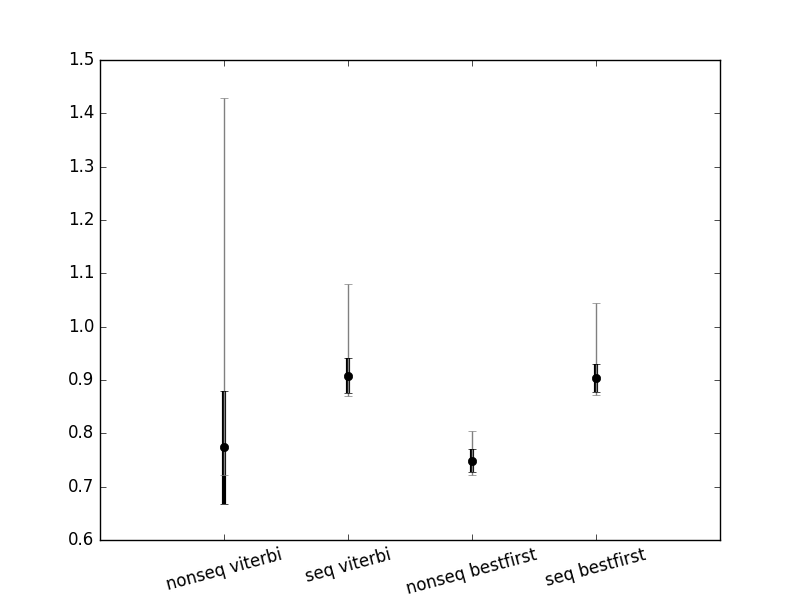
\includegraphics[width=0.90\linewidth]{fit_time.png}
	\label{fit-time}
	\caption{Czas uczenia (w ms)}
\end{figure}

\newpage

Kolejnym badaniem było sprawdzenie czasu testowania. Tutaj już widać znaczący, bo aż blisko 10-krotny wzrost czasu testowania zbioru sekwencyjnego względem zbioru bazowego. Różnice między algorytmami również nie są bardzo widoczne, zauważyć jednakże również można mniejszy rozrzut algorytmu \textit{best-first}.

\begin{table}[ht!]
\centering
\caption{Wyniki badań - czas testowania (w ms)}
\label{my-label}
\begin{tabular}{|c|c|c|c|c|}
\hline
\textbf{}     & \textbf{nonseq Viterbi} & \textbf{seq Viterbi} & \textbf{nonseq best-first} & \textbf{seq best-first} \\ \hline
\textbf{min}  & 0.1368                  & 1.1994               & 0.1366                     & 1.3415                  \\ \hline
\textbf{max}  & 0.2546                  & 1.7130               & 0.1640                     & 1.4338                  \\ \hline
\textbf{mean} & 0.1445                  & 1.2293               & 0.1418                     & 1.3628                  \\ \hline
\textbf{std}  & 0.0133                  & 0.0607               & 0.0050                     & 0.0157                  \\ \hline
\end{tabular}
\end{table}

\begin{figure}[h!]
	\centering
	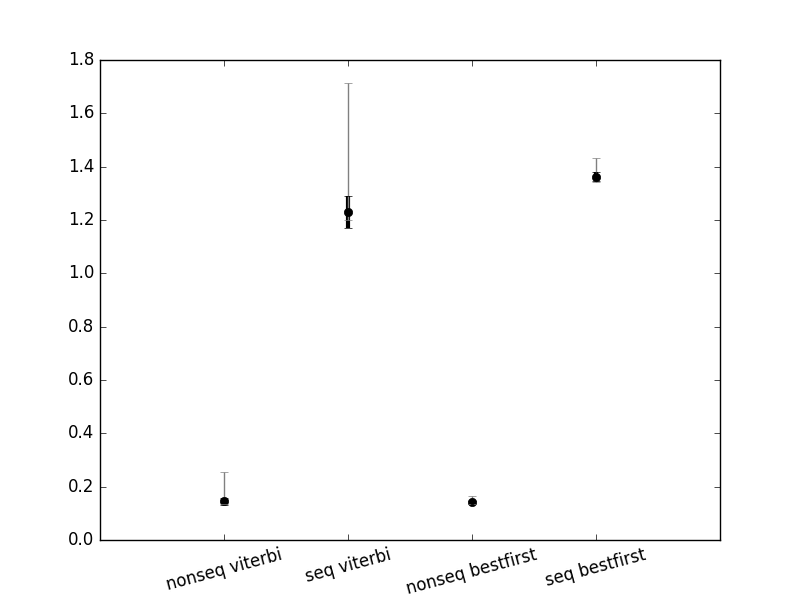
\includegraphics[width=0.90\linewidth]{score_time.png}
	\label{score-time}
	\caption{Czas testowania (w ms)}
\end{figure}

\newpage

Ostatnim przeprowadzonym eksperymentem było sprawdzenie efektywności modelu. Zauważyć można, iż na efektywność nie ma wpływu rodzaj zastosowanego zbioru, a wręcz zauważyć można, że dla zbioru sekwencyjnego rośnie rozrzut wartości względem zbioru bazowego, co sugeruje jego mniejszą stabilność. Różnice między dwoma algorytmami są także prawie niezauważalne.

\begin{table}[ht!]
\centering
\caption{Wyniki badań - dokładność (w \%)}
\label{my-label}
\begin{tabular}{|c|c|c|c|c|}
\hline
\textbf{}     & \textbf{nonseq Viterbi} & \textbf{seq Viterbi} & \textbf{nonseq best-first} & \textbf{seq best-first} \\ \hline
\textbf{min}  & 56.8965                 & 54.3859              & 56.8965                    & 45.6140                 \\ \hline
\textbf{max}  & 82.7586                 & 87.7192              & 82.7586                    & 86.8421                 \\ \hline
\textbf{mean} & 70.9827                 & 68.1140              & 70.2931                    & 68.2456                 \\ \hline
\textbf{std}  & 5.5390                  & 7.7356               & 5.0435                     & 9.6267                  \\ \hline
\end{tabular}
\end{table}

\begin{figure}[h!]
	\centering
	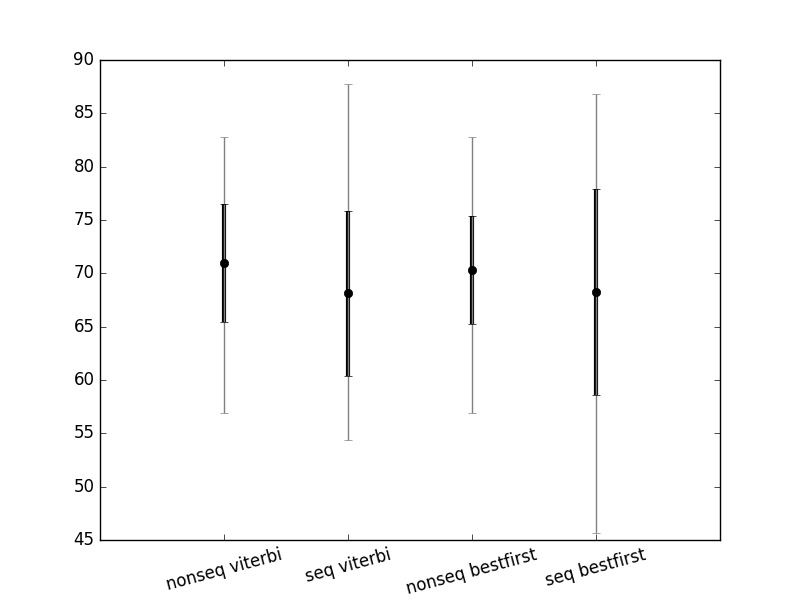
\includegraphics[width=0.90\linewidth]{accuracy.png}
	\label{accuracy}
	\caption{Dokładność (w \%)}
\end{figure}
    %\newpage

\section{Podsumowanie}

    
    %\newpage
    %\bibliographystyle{plabbrv}
    %\nocite{*}
    %\bibliography{bibliografia}

\end{document}
